%% 卒業論文概要原稿用テンプレート
\documentclass[twocolumn]{jsarticle}
%% パッケージの設定
\usepackage[dvipdfmx]{graphicx}
\usepackage{mseproc}
\usepackage{amssymb,amsmath}
\usepackage{bm}
\usepackage{url}

%% 学科名・発表番号
\renewcommand{\mplab}{□□□□□□研究室}
\renewcommand{\mpcode}{☆--10}
%% 和文題目
\renewcommand{\mpjtitle}{
  卒業論文概要原稿用\LaTeXe テンプレート
}
%% 指導教員名・学籍番号・著者名
\renewcommand{\mpsupervisor}{○○~○○~教授}
\renewcommand{\mpsid}{0123456}
\renewcommand{\mpauthor}{△△~△△}

\begin{document}
\btitle

\section{このテンプレートについて}
このファイル\texttt{undergraduate2023.tex}は,
東京都市大学理工学部機械システム工学科の
卒業論文概要原稿を\LaTeXe で作成するためのテンプレートです.
基本事項はすべて,Wordのテンプレート\cite{msetemplateB}
を参照し,\LaTeXe で作成する場合の書式に必要な部分を
このテンプレートに合わせてください.

\section{使用するための前提条件}
使用条件として下記を前提としています.
\begin{enumerate}
\item \LaTeXe にある程度習熟している\cite{Okumura2023}.
\item \pLaTeXe がインストールされている. %(\ref{sec:latexinstall}節参照).
\item \texttt{jsarticle.cls}がインストールされている\cite{Okumura2023}.
\end{enumerate}

テンプレート作成と動作確認は,Overleaf上で実施しました.
Overleaf上でのコンパイルのために
このファイルと一緒に配布している設定ファイル
\texttt{latexmkrc}が同じディレクトリ内に存在する必要があります.
また,機械システム工学領域の指定書式に従うため,
\texttt{mseproc.sty}も同一ディレクトリ内に置いてください.

WindowsやLinux上で利用可能な\LaTeXe の統合環境での
動作確認は行っていません.
もし利用時に何か問題があった場合は,Word用テンプレートに記載された
概要原稿の基本の書式を守った上で適宜修正をお願いします.
また,文字コードはUTF-8です.
Windows上での利用の際は,Shift-JISに変換することが必要かもしれません.
なお,この後の説明文中に出てくるバックスラッシュ記号\verb+\+は,
円マーク記号(半角の\yen)と同一です.


\section{テンプレートの使用方法}
まずプリアンブル
\footnote{\verb+\begin{document}+の前}
の下記項目を注意深く設定してください.

\subsection{研究室名・論文番号}
左上に所属研究室名と論文番号を表記するため,
\verb+\renewcommand{\mplab}{研究室名}+,\\
\verb+\renewcommand{\mpcode}{☆--00}+ \\
の2カ所をTable~\ref{table:lablist}に従って書き変えます.
☆印をローマ数字に置き換えてください.
\LaTeX のハイフンは\verb+-+を2個続けて書く(\verb+--+)ことに注意しましょう.
%
\begin{table}[ht]
  \centering
  \caption{Lab. list in our department.}
  \label{table:lablist}
  \begin{tabular}{|l|l|}\hline
    I & 熱流体システム研究室 \\ \hline 
    II & 高機能機械制御研究室 \\ \hline
    III & ロボティックライフサポート研究室 \\ \hline 
    IV & 強度設計システム研究室 \\ \hline
    V & 計測電機制御研究室 \\ \hline
    VI & 宇宙システム研究室 \\ \hline
  \end{tabular}
\end{table}

\subsection{論文題目}
\verb+\renewcommand{\mpjtitle}{...}+
を設定します.

\subsection{指導教員名}
\verb+\renewcommand{\mpsupervisor}{...}+ \\
を設定します.

\subsection{学籍番号}
\verb+\renewcommand{\mpsid}{...}+
を設定します.

\subsection{著者名}
\verb+\renewcommand{\mpauthor}{...}+
を設定します.

\subsection{タイトル部の表示}
上記のプリアンブルの項目をすべて設定した後,
\verb+\begin{document}+の後で\verb+\btitle+を設定すれば,
フォーマットに合わせたタイトル部が表示されます.

\subsection{本文の記述}
上記を確認したら\texttt{undergraduate2023.tex}を適宜編集してください.


\section{利用上の注意}

\subsection{\texttt{jsarticle.cls}について}
このテンプレートを作者が意図した通りに利用するためには,
\texttt{jsarticle.cls}\cite{Okumura2023}が必要であり,
基本的な書式はその仕様に依存します.
したがって,\texttt{jsarticle.cls}のバージョンが違う場合は
結果が多少異なる可能性があるので注意してください.
また,文字のデフォルトの大きさを変更することは避けましょう.
例えば12ptに変更すると,\verb+\hspace*{10mm}+が12~mmの空白になることがあります.

\subsection{PDFファイルへの変換について}
原稿はPDFファイルで提出してください.
写真や図にビットマップイメージを用いている場合は
PDFファイルに変換した後の図の解像度やファイルサイズに注意しましょう.
%PDFへの変換方法については\ref{dvipdf}節で簡単に説明しますが,
%環境が異なる場合は文献\cite{Kagi,TeXWiki}などを参照し,各自で対応してください.
OverleafやWinShellなどの統合環境ではメニューにPDFへの変換機能が用意されています.
作成したPDFは機械システム工学科の指定書式に適しているかを確認後に提出してください.


% Overleafでの確認のみのため,環境構築については割愛しました.
%
% \section{環境構築}
% \label{sec:latexinstall}
% Windows XP上での環境構築の指針を示す.

% \subsection{\LaTeXe インストール}
% \subsubsection{TeXインストーラ3}
% 「TeXインストーラ3」\cite{texinstaller}を用いると
% 一通りのソフトウエアを自動的にインストール・設定できる.
% Plug-inを導入することでWinShellのインストールと環境設定も
% 行うことができる.
% インストール時にブロードバンド環境を必要とする.
% \subsubsection{美文書作成入門付属のCDを用いる}
% 文献\cite{Okumura2000}に付属のCDで一通りインストールできるが,
% 最新版ではないこともある.

% \subsection{エディタや統合環境}
% \subsubsection{\texttt{Winshell}}
% \texttt{Winshell 3}をインストールすればGUIの統合環境を構築できる
% \cite{TeXWiki}.
% 美文書作成入門\cite{Okumura2000}のCDにも入っているが最新版ではない
% 可能性がある.
% \subsubsection{\texttt{Akasha}}
% シェアウエアの使いやすいGUI統合環境.文献\cite{TeXWiki}のTeX用エディタを参照.
% \subsubsection{\texttt{サクラエディタ}}
% 評判の良いエディタ.文献\cite{TeXWiki}を参照.
% \subsubsection{\texttt{Meadow/Emacs+AUCTeX/YaTeX}}
% 有名なエディタと\LaTeXe の入力支援環境.マウスを使わずに
% タイプセットできる.
%
% \subsection{PDFへの変換}
% \label{dvipdf}
% texファイルをタイプセットして作成したdviファイルは下記の方法で
% PDFファイルに変換できる.2番目以降はコマンドプロンプトの操作を
% 必要とする.
%
% \subsubsection{統合環境}
% WinshellやAkashaなどの統合環境の多くはPDFへの変換メニューを用意している.
% \subsubsection{\texttt{dvipdfmx}}
% dviからpdfに変換する.詳しくは文献\cite{TeXWiki}を参照.
% \subsubsection{Adobe Acrobat}
% まず\texttt{dvipsk}を用いてPSファイルに変換する.
% \begin{verbatim}
%   > divpsk -Ppdf -t a4 xxx.dvi
% \end{verbatim}
% 次にAdobe AcrobatでPDFファイルに変換する
% \footnote{Acrobat Elements以上で変換できる.Adobe Readerでは変換できない.}
% .文献\cite{TeXWiki}を参照すること.


\section{数式の書き方}

\subsection{数式の記述に関する注意}
式には番号を付けます.
\begin{equation}
  \bm{M} \ddot{\bm{q}} + \bm{C}(\bm{q},\dot{\bm{q}}) 
  + \bm{D} \dot{\bm{q}} + \bm{G}(\bm{q}) = \bm{\tau}
  \label{eqn:manipulatoreqs}
\end{equation}
式を並べる場合は次のようにします.
\begin{eqnarray}
  \dot x & = & A x + B u \\
  y & = & C x + D u
\end{eqnarray}

\subsection{数式の参照}
上の最初の方程式を参照するには,\verb+\ref+を用いて
(\ref{eqn:manipulatoreqs})とします.

\subsection{文章中の数式の記述}
文章中に数式を書く場合は,p=0 ではなく,\verb+$p=0$+と書いて
$p=0$と出力します.
分数を書く場合には,$\frac{y}{x}$ ではなく,$y/x$としてください.

\subsection{三角関数・対数関数など}
三角関数を\verb+$sin$+と書くと,
三つの文字を掛け合わせる$s\times i\times n$の意味の$sin$となってしまいます.
\verb+$\sin$+と書けば$\sin$と正しく出力されます.他にも
$\cos$,$\tan$,$\log$など一般的な数学関数はコマンドが用意されています.


\section{表の書き方}
表を書く場合はTable~\ref{table:jitter}のようにしましょう.
\begin{table}[ht]
  \centering
  \caption{Scheduling jitter data.}
  \label{table:jitter}
  \begin{tabular}{|c|c|c|}\hline
    & Maximum [$\mu$s] & Average [$\mu$s] \\ \hline \hline
    Standard kernel & $2.06 \times 10^3$ & $1.45 \times 10^3$ \\ \hline
    Real-time kernel & 92.0 & 25.5 \\ \hline
  \end{tabular}
\end{table}


\section{図の取り込み}
\LaTeXe 文書に挿入する図のファイル形式はPDFを推奨します.
ほかにEPS,JPEG,PNG形式のファイルも利用できますが,
図の解像度やファイルサイズに注意しましょう.

\subsection{図の記述}
図中の語句やキャプションは必ず英語で記述してください.
図の幅の指定値は最大で80~mmとします.
長さ変数の\verb+\figurewidth+を用意してあり,
これを用いると自動的にcolumnの幅いっぱいに表示されます.
例:\\
{\small \verb+\includegraphics[width=\figurewidth,clip]{...}+}

\subsection{図の参照の例}
Fig.~\ref{fig:snapthru}は,2次遅れ系
%
\begin{equation}
  \frac{Y(s)}{U(s)} = \frac{K\omega_n^2}{s^2+2\zeta \omega_n s + \omega_n^2}
\end{equation}
%
について,$K=\omega_n=1$の下で減衰係数$\zeta$を
$\zeta=2,1$,$0.8$,$0.6$,$0.4$,$0.2$,$0$とした場合の
単位ステップ応答波形です.
%
\begin{figure}[tb]
  \centering
  \includegraphics[width=0.8\linewidth]{fig/StepResponse.eps}
  \caption{Step response of second order systems: 
    damping coefficient affects convergence speed.}
  \label{fig:snapthru}
\end{figure}

\subsection{図の配置}
Floatingパラメータを調整してあるため,
意図した場所に入ると思いますが,
入らなかった場合には図の大きさや位置を調整してください.
また,好みもありますが,図表はすべて,
\verb+\begin{figure}[t]+,
\verb+\begin{tabule}[t]+
とすれば,きれいに配置できます.

\section{図の作成に関する注意}
EPSファイルを作成する際に注意することは,
図の種類がベクトルグラフィックスか
ビットマップグラフィックスかの違いを意識して
EPSファイルを作成することです.
グラフ・ブロック線図などは前者いなり,
写真は後者になります.
このことを意識せずにデータを作ると,
見苦しいグラフや巨大なEPSファイルを作ることになります.
Fig.~\ref{fig:ComparingEPS}に例を示すので拡大して比較してみましょう.
(説明のためにFig.~\ref{fig:ComparingEPS}のキャプションは
日本語としましたが,概要原稿の図説は必ず英語で記載してください.)
%
\begin{figure}[tb]
  \centering
  \begin{tabular}[t]{cc}
    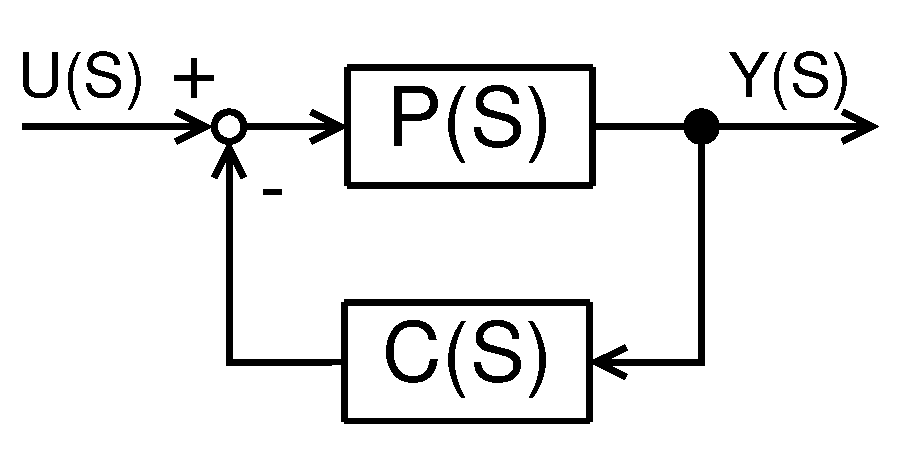
\includegraphics[width=0.65\linewidth]{fig/Feedback.eps} \\
    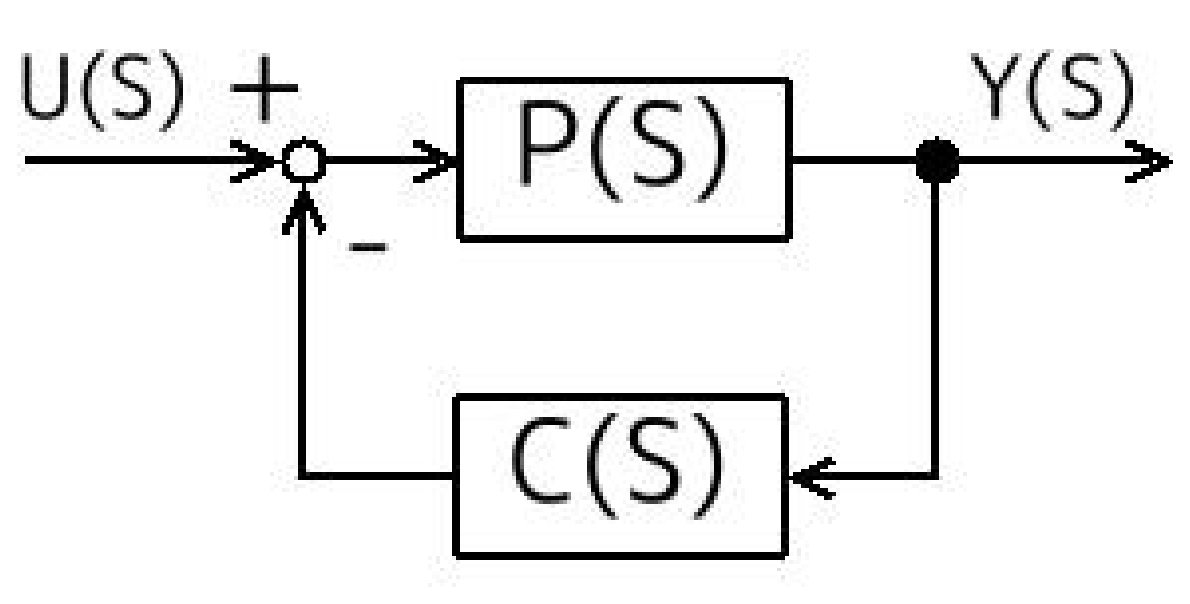
\includegraphics[width=0.65\linewidth]{fig/Feedback-jpeg.eps}
  \end{tabular}
  \caption{diaを用いてベクトルデータで作成したブロック線図:
    上はベクトルEPS,
    下はビットマップEPS(JPEGファイルで保存しjpeg2psを用いてEPSに変換したもの).
    下図ではエイリアスが発生しています.}
  \label{fig:ComparingEPS}
\end{figure}

以下では,図の種類ごとにEPSファイルを作成するための指針を示します.
ツールの詳細は文献\cite{TeXWiki}の「変換ツール」を参照してください.

\subsection{グラフ}
gnuplotやExcelなどを使用して作成します.

\subsubsection{gnuplot}
gnuplotの使用法は文献\cite{GnuplotPerfect,GnuplotTP}に詳しく説明されています.
次のようにコマンド入力すると,\texttt{foo.eps}が作成されます.
\begin{verbatim}
> set terminal postscript eps
> set output "foo.eps"
> replot
\end{verbatim}
EPSファイルのフォントサイズを20ポイントにする場合は,
ターミナル設定で次のように入力します
\footnote{texで図をスケールするとフォントサイズも変化することに注意しましょう.}.
\begin{verbatim}
> set terminal postscript eps 20
\end{verbatim}

\subsubsection{Excel}
Microsoft 365のExcelの図は, Metafile to EPS Converter
(\url{https://wiki.lyx.org/Windows/MetafileToEPSConverter})を
利用するとベクトルデータのままでEPSに変換できます.
設定などの詳細は文献\cite{Metafile2EPSConverter} を参照してください.

\subsection{ブロック線図などの図}
Fig.~\ref{fig:block}のような,
線や円を中心としたベクトルデータの図形は
OpenOffice.orgのDrawや
Visio, PowerPointなどを使用して作成します.
DrawではEPSを直接作成できます.
また前述のMetafile to EPS Converterを用いると
Microsoft 365の図をEPS形式にして保存できます.
% 
\begin{figure}[tb]
  \centering
  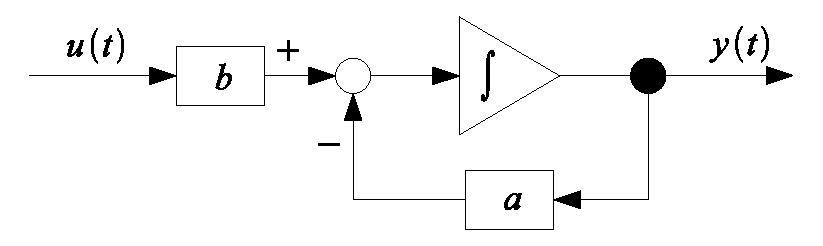
\includegraphics[width=0.9\linewidth]{fig/SFDiagram.eps}
  \caption{Example of a state flow diagram depicted with ``OpenOffice.org Draw.''}
  \label{fig:block}
\end{figure}

\subsubsection{Metafile to EPS Converter}
Metafile to EPS Converterを用いると
PowerPointやVisoで作成した図もコピーアンドペーストで
EPS形式にして保存できるため,
Windows上では大変便利です\cite{Metafile2EPSConverter}.
% \subsubsection{VisioとPowerPoint(wmf形式)}
% WMF形式のファイルは,
% Metafile to EPS Converterを利用するとベクトルデータのまま
% EPSに変換できます.

\subsubsection{OpenOffice.org Draw}
OpenOffice.orgのDrawを用いると高品質のベクトルデータのEPSを
直接作成できます.保存する際にオブジェクトを選択し,
選択範囲をEPSとしてエクスポートすればよいです
(\url{https://www.openoffice.org/ja/}).

% 開発が止まっているため削除しました.
% \subsubsection{dia}
% ベクトルデータのEPSファイルを直接作成できます
% (\url{http://www.gnome.org/projects/dia/}).

\subsubsection{PDF形式とAdobe Acrobatを用いた変換}
PDF形式で出力した後に,
Adobe Acrobatを利用して編集をすることで
範囲を選択した後にEPSファイルとして保存ができます.
Visioではアドインを利用すればPDFで保存でき,
Acrobatから直接EPSを選択してdvioutがエラーを
発生する場合は,PSファイルに一度保存し,
Photoshopなどで再度EPSファイルに保存すると良いです.

\subsection{写真など}
JPEGファイルは,\texttt{jpeg2ps}を用いると
画像の品質を損なうことなく,
サイズもほとんど同じEPSファイルに変換できます.
例:
\begin{verbatim}
  > jpeg2ps foo.jpg -o foo.eps
\end{verbatim}

\subsection{Linux上のツール}
tgif, xfigなど,Linuxでは\LaTeXe やEPSなどに対応したツールが充実しています.


\section{プログラムのコードをそのまま出力する方法}
プログラムのソースコードを\LaTeXe で表示する場合は
\verb+verbatim+環境を用います.
\verb+\begin{verbatim}+と\verb+\end{verbatim}+の間は,
以下のように\TeX の文字が空白も含めてそのまま表示されます.
\begin{verbatim}
#include <stdio.h>
int main()
{
   printf("Hello, world\n");
   return 0;
} 
\end{verbatim}


\section{書式に関する注意}
\LaTeXe による文書作成では改段落の方法の誤りをよく目にします.
日本語の文章では文章の区切りで改行し,
新しい行の先頭は全角1文字分の空白を入れるようにしましょう.
ここからは,.texファイルに書かれている内容を直接確認してください.
例えば,この文を段落の終わりとします.

次の段落はこのように始まる.\LaTeXe でこれを実現するには,
\texttt{tex}ファイルに改行命令\verb+\\+を入れるのではなく,
ただ,空行を1行入れて改行し,
先頭に1文字分の空白を入れずに次の段落の文章を始めればよいです.
この書き方を習得しましょう.

なお,\verb+\section+コマンドの後の文章は段落の
始まりと考えられるので,行の先頭に自動的に空白が入ります.
そのほかに下記に注意してください.
\begin{itemize}
\item 文章中の英数字や記号は全角ではなく半角で記述する.
  例えば,``2006年''ではなく``2006年''とし,
  ``MSE''ではなく``MSE''とします.
\item 句点:``。``ではなく''.``を用います.
\item 読点:``、``ではなく'',``を用います.
\end{itemize}

{\small
\begin{thebibliography}{99}
\bibitem{msetemplateB}
  (2023, Jan. 30)機械システム工学科:
  ``卒業論文概要原稿の書き方'',
  東京都市大学~理工学部.[Online].
  Available: \url{http://www.mse.tcu.ac.jp/defense.html}
\bibitem{Okumura2023}
  奥村晴彦,黒木祐介:
  ``[改訂第9版]\LaTeX 美文書作成入門'',
  技術評論社,2023.
\bibitem{LaTeXeBook}
  中野賢:
  ``日本語\LaTeXe ブック'',
  アスキー出版局,1996.
\bibitem{GnuplotPerfect}
  川原稔:
  ``Gnuplotパーフェクトマニュアル'',
  SBクリエイティブ, 1999.
\bibitem{GnuplotTP}
  矢吹道郎,大竹敢:
  ``使いこなすGnuplot'',
  Techno Press, 2000.
\bibitem{Kagi}
  (2023, Jan. 30)物理のかぎしっぽ.[Online].
  Available: \url{http://hooktail.org/computer/index.php?TeX}
\bibitem{TeXWiki}
  (2023, Jan. 30)\TeX \texttt{Wiki}. [Online].
  Available: \url{https://texwiki.texjp.org/}
% Websiteがアクセスできないため削除しました.
% \bibitem{texinstaller}
%   (2009, Dec. 7) TeXインストーラ3のダウンロード.[Online].
%   Available: \url{http://www.ms.u-tokyo.ac.jp/~abenori/mycreate/index.html}
\bibitem{Metafile2EPSConverter}
  (2023, Jan. 30)Metafile to EPS ConverterでWindows MetafileをEPSに変換.
  Available: \url{https://qiita.com/tubo28/items/1f8672fb164aafa9ab31}
\end{thebibliography}

\appendix
\section{更新履歴}
%%最終更新 \today\\
\begin{tabular}[t]{|l|l|l|} \hline
  版 & 更新日 & 備考 \\ \hline \hline
  1.0 & 2001/12/15 & 初版 \\ \hline
  1.1 & 2001/12/25 & 数学記号を追記 \\ \hline
  1.2 & 2001/12/28 & \verb+\section+フォント修正 \\
  & & \verb+\figurewidth+を設定 \\ \hline\hline
  2.0 & 2007/01/07 & 2006年度版に対応 \\
  & & 最近のソフトウエアを紹介 \\
  & & 研究室名の改行を防止 \\
  & & 図見出しの空白を短縮 \\
  & & 1節の見出し前の \\
  & & 空行を削除 \\ \hline
  2.1 & 2007/01/10 & 図の空白を調整 \\
  & & グラフを入れ替え \\
  & & 1節の見出しの \\
  & & フォントを修正 \\ \hline
  2.2 & 2008/05/05 & DrawとPDFによる \\
  & & 作図を加筆 \\ \hline
  2.3 & 2008/06/12 & \TeX インストーラ \\
  & & plug-inを加筆 \\ \hline
  2.4 & 2009/12/07 & \verb+wmf2eps+について詳しく追記 \\
  & & \verb+verbatim+環境を追加 \\ \hline\hline
  3.0 & 2011/08/25 & 2011年度版に改訂 \\ \hline
  3.1 & 2015/08/24 & Abstract, Key words, \\
  & & 参考文献を\\
  & & 9 pt (small)に変更 \\ \hline
  3.2 & 2023/01/30 & 2023年度版に改訂 \\ \hline
\end{tabular}

\end{document}

%%% Local Variables: 
%%% End: 
